\documentclass{beamer}
\usepackage[utf8]{inputenc}
\usepackage{graphicx}

\title{Webapplikation zur Erstellung und Ausgabe von Mathematikaufgaben}
\subtitle{Abschlussprojekt GymInf Weiterbildung}
\author{Oliver De Capitani und Patrick Weber}
\date{\today}

\begin{document}

% Titelblatt
\frame{\titlepage}

% Inhaltsverzeichnis
% \section*{Inhaltsverzeichnis}
% \begin{frame}{Inhaltsverzeichnis}
%     \tableofcontents
% \end{frame}

% Kapitel: Einleitung
\section{Einleitung}
\begin{frame}{Einleitung}
    \begin{itemize}
        \item<1-> Ziel: Entwicklung einer Webapplikation, um Mathematikaufgaben zu erstellen, zu verwalten und herunterzuladen.
        \item<2-> Inspiration: Frühere Plattform munterbunt.ch.
        \item<3-> Anforderungen:
        \begin{itemize}
            \item Benutzerregistrierung und Login.
            \item Aufgaben filtern, sammeln und im Tex-Format herunterladen.
            \item Eigene Aufgaben erstellen, bearbeiten oder löschen.
        \end{itemize}
        \item<4-> Technologie-Stack: Full-Stack-Entwicklung mit Docker, React/Preact, Prisma und PostgreSQL.
    \end{itemize}
\end{frame}

% Kapitel: Struktur der Webapplikation
\section{Struktur der Webapplikation}
\subsection{Architekturübersicht}
\begin{frame}{Architekturübersicht}
    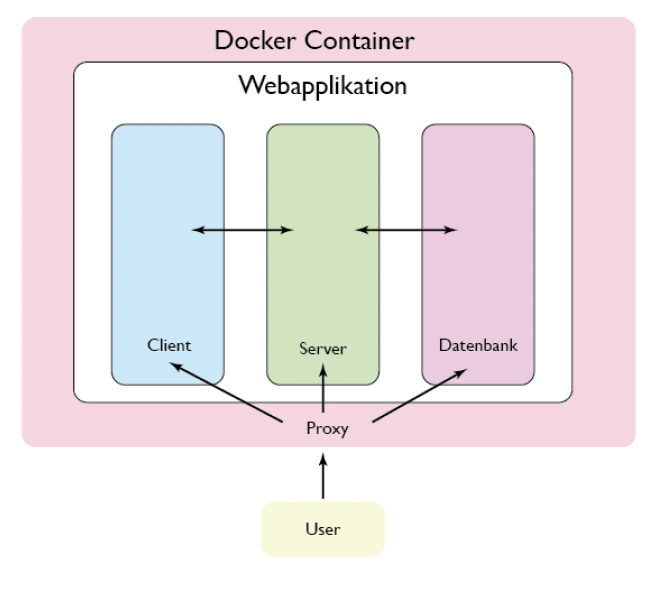
\includegraphics[width=0.5\textwidth]{docker_overview.png}
    \begin{itemize}
        \item Anwendung läuft in einem Docker-Container.
        \item Proxy vermittelt zwischen Client, Server und Datenbank.
        \item Sicherheit: HTTPS über selbstsignierte Zertifikate.
    \end{itemize}
\end{frame}

\subsection{Technische Details}
\begin{frame}{Technische Details}
    \begin{itemize}
        \item \textbf{Server:}
        \begin{itemize}
            \item Express.js zur Verarbeitung von Anfragen.
            \item Passport.js für Authentifizierung.
            \item Prisma ORM für Datenbankoperationen.
        \end{itemize}
        \item \textbf{Datenbank:} PostgreSQL mit Prisma ORM.
        \item \textbf{Frontend:} React/Preact mit Komponentenhierarchie.
        \item \textbf{Deployment:} Docker-Container auf einem Linode-Server.
    \end{itemize}
\end{frame}

\subsection{Workflow der Anwendung}
\begin{frame}{Workflow der Anwendung}
    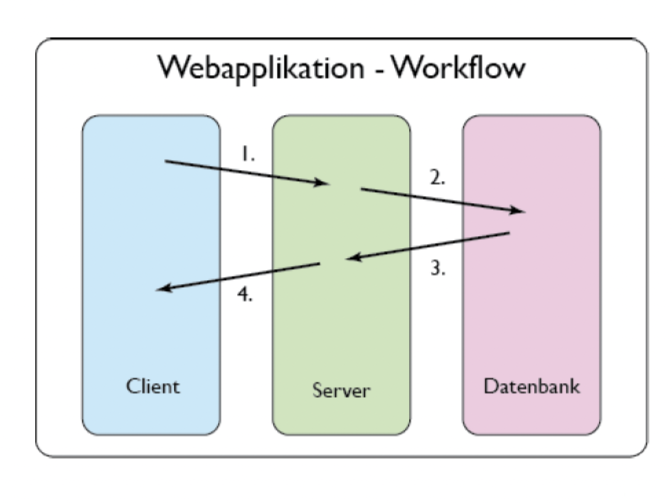
\includegraphics[width=0.6\textwidth]{workflow.png}
    \begin{enumerate}
        \item Nutzeranfrage (z. B. Download einer Aufgabe) wird an den Server gesendet.
        \item Server fragt die Datenbank ab und verarbeitet die Ergebnisse.
        \item Die resultierenden Daten werden an den Client zurückgegeben.
    \end{enumerate}
\end{frame}

% Kapitel: Datenbank
\section{Datenbank}
\begin{frame}{Datenbankstruktur}
    \begin{itemize}
        \item Tabellen:
        \begin{itemize}
            \item \textbf{User:} Speichert Benutzerdaten und Login-Informationen.
            \item \textbf{Exercise:} Enthält Aufgabeninhalte und Metadaten.
            \item \textbf{Category/Subcategory:} Hierarchische Organisation von Aufgaben.
        \end{itemize}
        \item Beziehungen:
        \begin{itemize}
            \item 1:n Beziehung zwischen Benutzer und Aufgaben.
            \item n:1 Beziehung zwischen Aufgaben und Kategorien.
        \end{itemize}
    \end{itemize}
\end{frame}

% Kapitel: Client-Architektur
\section{Frontend-Architektur}
\begin{frame}{Frontend-Architektur}
    \begin{itemize}
        \item Komponenten:
        \begin{itemize}
            \item \textbf{AufgabenSuchen:} Filterung und Anzeige von Aufgaben.
            \item \textbf{AufgabeDetails:} Detaillierte Ansicht einer Aufgabe.
            \item \textbf{Warenkorb:} Verwaltung gesammelter Aufgaben.
            \item \textbf{AufgabeHinzufügen/Ändern:} Formulare zur Bearbeitung.
        \end{itemize}
        \item Zustandshandling:
        \begin{itemize}
            \item \texttt{useContext}: Globaler Zustand für Suche und Warenkorb.
            \item \texttt{useState}, \texttt{useEffect}: Lokale Zustandsverwaltung.
        \end{itemize}
    \end{itemize}
\end{frame}

% Kapitel: Prozess und Herausforderungen
\section{Prozess und Herausforderungen}
\subsection{Koordination}
\begin{frame}{Koordination}
    \begin{itemize}
        \item Nutzung von Trello zur Planung und Aufgabenverteilung.
        \item Agile Kommunikation im kleinen Team.
        \item Herausforderung: Übersichtlichkeit und Priorisierung in der Anfangsphase.
    \end{itemize}
    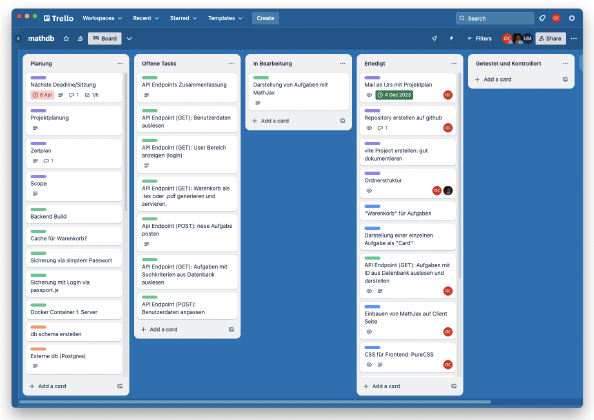
\includegraphics[width=0.6\textwidth]{trello_screenshot.png}
\end{frame}

\subsection{Probleme und Lösungen}
\begin{frame}{Probleme und Lösungen}
    \begin{itemize}
        \item \textbf{CORS-Probleme:}
        \begin{itemize}
            \item Ursache: Anfragen an unsichere Domains.
            \item Lösung: Spezifikation erlaubter Domains im Server-Code.
        \end{itemize}
        \item \textbf{Testdatenbank:}
        \begin{itemize}
            \item Ursache: Konflikte durch manuell gesetzte IDs.
            \item Lösung: Automatische ID-Zuweisung.
        \end{itemize}
    \end{itemize}
\end{frame}

% Kapitel: Zusammenfassung und Ausblick
\section{Zusammenfassung und Ausblick}
\begin{frame}{Zusammenfassung}
    \begin{itemize}
        \item Umsetzung der Kernfunktionen:
        \begin{itemize}
            \item Aufgaben filtern, sammeln, herunterladen.
            \item Benutzerregistrierung und Login.
        \end{itemize}
        \item Lernprozess: Vertieftes Verständnis von Full-Stack-Entwicklung.
    \end{itemize}
\end{frame}

\begin{frame}{Ausblick}
    \begin{itemize}
        \item Erweiterungen:
        \begin{itemize}
            \item Benutzerprofile und Filtermöglichkeiten.
            \item Integration weiterer Fachbereiche.
            \item Kommentarfunktion für Aufgaben.
        \end{itemize}
        \item Verbesserung der Codebasis für Skalierbarkeit.
    \end{itemize}
\end{frame}

% Abschlussfolie
\section*{Danke}
\begin{frame}{Danke!}
    \centering
    Vielen Dank für Ihre Aufmerksamkeit! \\
    \vspace{1cm}
   
\end{frame}

\end{document}
